\chapter{\textsc{Methodology}}
\label{chapter:methodology}

This chapter extends the Methodology section in Chapter \ref{chapter:project_design}: Project Design. Firstly, it provides an introduction to the EPSRC grant data used in this project and details its collection process. Secondly, the networks generated from the collected EPSRC data are introduced. Thirdly, the tools used in this project are presented and their use is highlighted. Furthermore, the contrast between grants as edges and grant records is outlined. Additionally, the process of formulating the node and edge attributes is presented, together with the normalisation process of the attribute values. Finally, the common experiment settings employed in all experiments are specified and the experiment process in which several edge weight interpretations and community detection algorithms are interchangeably tested is briefly described.

\section{EPSRC grant data}

This project uses data provided publicly by EPSRC through the \textit{EPSRC GoW} service. It consists of current and historical data stored within the \textit{Current} and \textit{Past Grant Portfolio}, respectively.

\subsection{EPSRC GoW service}

The \textit{GoW} service is a web-based facility providing information about research grants funded by EPSRC. The service is updated frequently, and consists of large amounts of information regarding historical and current grants, researchers, panels and quarterly summaries. It also includes search functionality allowing users to search the Web database.

\subsection{EPSRC Current and Past Grant Portfolio}

The \textit{Current} and \textit{Past Grant Portfolio} are sub-facilities of the \textit{GoW} service providing access to current and historical grant data. Both facilities provide the same kind of information, however the access to information differs slightly. The \textit{Past Grant Portfolio} requires a time period to be supplied, and provides grants based on it. This can be a start date, an end date or a start and end date. Fig. \ref{fig:current_grant_portfolio} and Fig. \ref{fig:past_grant_portfolio} present the hierarchical structure of the EPSRC \textit{Current} and \textit{Past Grant Portfolio}, respectively.

\begin{figure}[htpb]
    \centering
    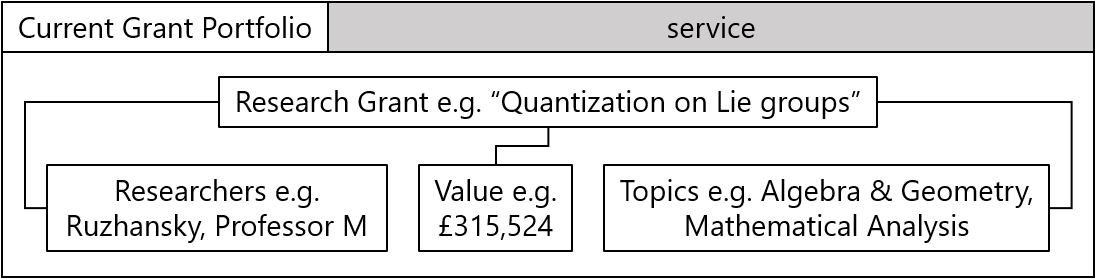
\includegraphics[width=10cm]{portfolios-explained/current_grant_portfolio}
    \caption{Hierarchical structure of the EPSRC Current Grant Portfolio.}
    \label{fig:current_grant_portfolio}
\end{figure}

\begin{figure}[htpb]
    \centering
    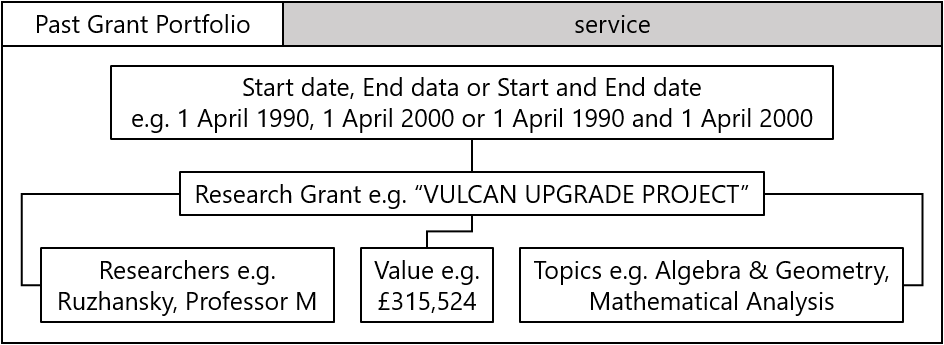
\includegraphics[width=10cm]{portfolios-explained/past_grant_portfolio}
    \caption{Hierarchical Structure of the EPSRC Past Grant Portfolio.}
    \label{fig:past_grant_portfolio}
\end{figure}

Each grant record is stored within a separate web page and contains details about the grant such as \textit{reference}, \textit{investigators (researchers)}, \textit{partners}, \textit{department}, \textit{organisation}, \textit{start} and \textit{end date}, \textit{value} and \textit{topic} and \textit{industrial sector classifications}. Fig. \ref{fig:grant_record} shows an example of a grant record within the \textit{EPSRC GoW} service.

\begin{figure}[htpb]
    \centering
    \fbox{
\includegraphics[width=12cm]{epsrc-records/grant_record}}
    \caption{Grant record in the \textit{EPSRC GoW} service.}
    \label{fig:grant_record}
\end{figure}

The researchers within each grant record are linked to separate researcher records. Each researcher record is also stored within a separate web page and contains details about the researcher including \textit{name}, \textit{organisation}, \textit{department}, \textit{current topics} and \textit{grants}. Fig. \ref{fig:researcher_record} shows an example of a researcher record within the \textit{EPSRC GoW} service.

\begin{figure}[htpb]
    \centering
    \fbox{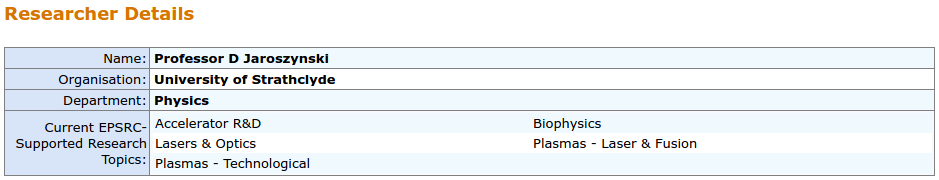
\includegraphics[width=12cm]{epsrc-records/researcher_record}}
    \caption{Researcher record in the \textit{EPSRC Grants on Web (GoW)} service.}
    \label{fig:researcher_record}
\end{figure}

\section{Collection of data from EPSRC}

The previous sections provided an introduction to the data provided by EPSRC, the \textit{Grants on the Web service (GoW)}, the \textit{Current} and \textit{Past Grant Portfolios} and the \textit{Grant} and \textit{Researcher} records. This project solely uses data collected from the \textit{Current} and \textit{Past Grant Portfolios}, and does not use any of the other information provided through the \textit{GoW} service. In terms of the \textit{Current} and \textit{Past Grant Portfolios}, this project only makes use of data extracted from grant and researcher records. 

Firstly, data within the following fields of a grant record was extracted:
\textit{EPSRC Reference}, \textit{Principal Investigator}, \textit{Other Investigators}, \textit{Starts}, \textit{Ends} and \textit{EPSRC Research Topic Classifications}. Secondly, data within the \textit{Name} and \textit{Current EPSRC-Supported Research Topics} fields of a researcher record was extracted.  Table \ref{table:grant_researcher_record_numbers} presents the number of current and historical EPSRC grant and researcher records from which data was collected.

\begin{table}[!htbp]
\renewcommand*{\arraystretch}{1.4}
\centering
\caption{Number of current EPSRC grant and researcher records and historical grant records from which data was collected.}
\label{table:grant_researcher_record_numbers}
\begin{tabular}{r|r|r|r}
{} & \multirow{2}{*}{\textbf{Current}}
& \multicolumn{2}{c}{\textbf{Historical}}\\
\cline{3-4}
& {} & \textbf{1990-2000} & \textbf{2000-2010}\\
\hline
\textbf{Number of Grant records}      & {3175} & {17861} & {18692}\\
\textbf{Number of Researcher records} & {5874} & {10820} & {13385}\\
\end{tabular}
\end{table}

\clearpage

\noindent Furthermore, the current and historical data used in this project is organised into two main data sets, while the historical data set is further divided into two sub-data sets as follows:

\begin{itemize}[noitemsep]
    \item \textbf{Current data set}, consisting of current (post 2010 start date) grant records collected on 8 July 2016 
    \item \textbf{Historical data set}, consisting of grant records from two time periods:
    \begin{itemize}
        \item \textbf{1990 to 2000}, consisting of grant records which started and ended between 1 April 1990 and 1 April 2000
        \item \textbf{2000 to 2010}, consisting of grant records which started and ended between 1 April 2000 and 1 April 2010
    \end{itemize}
\end{itemize}

As previously mentioned, both grant and researcher records are stored as separate web pages within the \textit{GoW} service. In order to extract content from a web page, a technique called \textit{web scraping} is employed. This is usually achieved by either using a third-party web scraper or by developing a web scraper from scratch, which extracts specified data from the underlying tags within the HTML code. In this case, a web scraper was developed using the \textit{requests} and \textit{lxml} Python libraries.

Essentially, the web scraper connects to the URL of each grant and researcher record and extracts the text found under specific fields such as \textit{Reference}, \textit{Principal Investigator} and \textit{Other Investigators}, \textit{Value} and \textit{EPSRC Research Topic Classifications}. Once extracted, the data is validated and then comma-delimited and text qualified using quotation marks which preserves its original format and allows easy manipulation of it. Subsequently, it is stored within comma-separated files categorised by content and data set.

\clearpage

\section{Generation of networks from EPSRC data}

The data extracted from the \textit{GoW} service was used to construct several networks of topics and researchers structured as follows:

\begin{enumerate}[noitemsep, label*=\arabic*.]
    \item \textbf{Networks of Topics, with nodes representing \underline{topics}}
    \begin{enumerate}[label*=\arabic*.]
        \item \textbf{Topic-grant network}, with edges representing \underline{grants};
            \begin{enumerate}[label*=\arabic*.]
                \item current version using the current data set (2010-2016)
                \item historical version using historical data set (2000-2010)
                \item historical version using historical data set (1990-2000)
            \end{enumerate}
        \item \textbf{Topic-researcher network}, with edges representing \underline{researchers};
            \begin{enumerate}[label*=\arabic*.]
                \item current version using the current data set (2010-2016)\footnote{The Topic (Nodes as Topics, Edges as Researchers) and Researcher network (Nodes as Researchers, Edges as Topics) were created using the Current data set only because Researcher records only consist of a researcher's current topics, and not their historical topics.}
            \end{enumerate}
    \end{enumerate}

    \item \textbf{Networks of Researchers, with nodes representing \underline{researchers}}
    \begin{enumerate}[label*=\arabic*.]
        \item \textbf{Researcher-grant network}, with edges representing \underline{grants};
        \begin{enumerate}[label*=\arabic*.]
                \item current version using the current data set (2010-2016)
                \item historical version using historical data set (2000-2010)
                \item historical version using historical data set (1990-2000)
            \end{enumerate}
        \item \textbf{Researcher-topic network}, with edges representing \underline{topics};
        \begin{enumerate}[label*=\arabic*.]
                \item current version using the current data set (2010-2016)\footnotemark[1]
        \end{enumerate}
    \end{enumerate}
\end{enumerate}

\section{Tools used in this project}

During this study, several tools were employed in order to accomplish various development and analysis activities. This section describes the tools and comments on their use throughout the project.

\subsection{JetBrains PyCharm for programming}

JetBrains PyCharm \cite{jetbrains_pycharm} is an Integrated Development Environment (IDE) for programming in Python. It also provides support for writing code in Bash. It was used to write the development code in primarily Python but also in Bash.

\subsection{Microsoft Excel for data storage}

Microsoft Excel \cite{microsoft_excel} is a spreadsheet software featuring calculation, graphing tools, pivot tables, and macro programming support in Visual Basic. It was used to explore, filter and validate the collected data.

\subsection{iGraph for network analysis and visualisation}

iGraph \cite{csardi2006igraph} is a library collection for creating and manipulating graphs and analyzing networks. This tool was used to compute network properties, apply community detection algorithms, and produce visualisations of the networks created.

\subsection{NetworkX for visualising adjacency matrices}

NetworkX \cite{networkx} is a package for the creation, manipulation, and study of the structure, dynamics and functions of complex networks in Python. It was used to visualise adjacency matrices.

\subsection{Wordle for creating word cloud visualisations}

Wordle \cite{wordle} is a tool for visualising text as word clouds. By default, it computes each word's frequency and displays the more frequent words in a larger font than less frequent ones. Additionally, Wordle's advanced mode allows keeping words together, specifying a weight which controls the font size, as well as specifying a colour for each word. It was to create word cloud representations of topic clusters using several attributes to control font size and colour.

\subsection{Adobe Photoshop for image editing}

Adobe Photoshop \cite{adobe_photoshop} is a graphics editor developed by Adobe Systems. It was used for image editing as well as turning network plots produced using iGraph into complete network visualisations.

\section{Common tasks}

A number of tasks were carried out for every network constructed using every data set, therefore, the tasks are considered common and are described in this section. They include identifying the contrast between grants as edges and grant record, the formulation of node and edge attributes and the normalisation of attribute values.

\subsection{Contrast between grants as edges and grant records}

It is essential to point out that there is a clear difference between grants represented by edges and the actual grant records that appear on the \textit{GoW} service. First and foremost, the former is not unique within a network, while the latter is unique within the \textit{GoW} service. This is due to the way links between topics or researchers were established in a network. If a pair of topics co-appear in X grants, the two will in theory be linked by M edges. In this study, the M edges are merged into a single edge between the two topics, and the weight of the edge is assigned as the total sum of the X grants. Essentially, if a grant is associated with N topics, N(N-1)/2 edges are created to link the N topics into a fully connected mesh graph. For example, if grant Y has 4 topics, 6 edges are created linking the topics into a 4-clique graph. Furthermore, it is also crucial to specify that unlike grants, a network consists of nodes representing unique topics.

This causes issues when questions like the following are posed: \textit{How many grants are in a specific community within a network's community structure?} \textit{What is the value of the grants?} It is important to mention that it is not known which grant is represented by an edge. It is only known that it represents one or more grants depending on the edge weight. If this was known, providing an answer to the above questions becomes significantly easier. In contrast, the answer was achieved through a lengthier process. Furthermore, the edges linking topics within the same community and the edges linking topics from different communities were known. This greatly aided the identification process of both the number and value of grants within communities and between communities.

Firstly, the origin and destination topics of an edge within a network were retrieved. Secondly, during the data collection process, a data structure was created which stored the reference of each grant record and the topics that classify it. Next, a check was carried out against all grant records which verified whether both the retrieved origin and destination topics appeared under a grant record. Number and value counters were created to keep track of the cumulative number and value of grants. If the check was true, the reference and value of the grant were added as the key and value to a Python dictionary, in which all keys must be unique. Finally, at the end of the check, the number of grant references was counted and the grant values were summed up. This provided an answer to the questions asked, as the number and value of grants within a community was successfully identified. Additionally, using the same technique, the computation of the number and value of grants between communities and within the entire network was also achieved. The function written in order to achieve this task is presented in Code snippet \ref{listing:turn_edges_into_grants}, part of Appendix \ref{appendix:code}.

\subsection{Formulation of node and edge attributes}

Every network constructed using the data collected from EPSRC consists of at least one node and edge attribute, while others consist of two attributes. Both \textit{Topic-grant} and \textit{Researcher-grant} networks consist of a \textit{number} and \textit{value} attribute, while the \textit{Topic-researcher} and \textit{Researcher-topic} networks only consist of a \textit{number} attribute. Visually, the network attributes control both the size of the node circle and the thickness of the edge line.

\subsubsection{Number of grants/topics/researchers}

The number attribute has a number of different contexts, depending on the network. Firstly, in the \textit{Topic-grant} and \textit{Researcher-grant} networks, the node number attribute represents the number of grants that a topic or researcher appears in. In the same networks, the edge number attribute represents the number of grants two topics or researchers have in common, meaning they both appear within the same grant record. Secondly, in the \textit{Topic-researcher} network, the node number attribute represents the number of researchers that a topic appears within, while the edge number attribute represents the number of researchers two topics have in common, meaning they both appear within the same researcher record. Thirdly, in the \textit{Researcher-topic} network, the node number attribute represents the number of topics a researcher currently has, while the edge number attribute represents the number of topics two researchers have in common.

\subsubsection{Value of grants}

Similarly, the value attribute also has a number of different contexts, depending on the network. Firstly, networks that are not based on grant data do not contain of the value attribute. Secondly, in the \textit{Topic-grant} and \textit{Researcher-grant} networks, the node value attribute represents the value of a topic or researcher. This represents the value of the grants that contain that specific topic or researcher. In the same network, the edge value attribute represents the value of the grants that two topics or researcher have in common, meaning they both appear within the same grant record.

\subsection{Normalisation of node and edge attribute values}

The numerical values used as the node and edge attributes, especially the value attribute, represent significantly large numbers which cause issues in terms of development, analysis and visualisation. To accommodate this, the values underwent a normalisation process which scaled the value range down. 
The function written in order to achieve this task can be viewed in Code snippet \ref{listing:norm_vals}, part of Appendix \ref{appendix:code}.

\clearpage

\noindent Furthermore, the formula used to normalize the values is presented below:

\begin{equation}
    (val - old\_min) \times new\_range / old\_range) + new\_min)
\end{equation}
where:
\begin{itemize}[noitemsep]
    \item \textit{val} is the value being normalised
    \item \textit{old\_min} is the minimum of the initial value range
    \item \textit{new\_range} is the new range values will be normalised to
    \item \textit{old\_max} is the maximum of the initial value range
    \item \textit{new\_min} is the minimum of the new value range
\end{itemize}

\section{Common experiments settings}

Extensive comparison experiments were conducted with the purpose of identifying an optimal solution for the data used in this project. An optimal solution is represented by a combination of an edge weight interpretation and a community detection algorithm. All candidates were tested on all networks, interchangeably. This means that each community detection algorithm was applied to each network constructed using each edge weight interpretation. The testing criteria is initially based on modularity score and community size. Later, the actual clusters are manually evaluated based on coherence and balance. In total, three different edge weight interpretations and eight different community detection algorithms are considered.

\subsection{Edge weight interpretations}

Previously, the process carried out to normalise the values used as node and edge attributes was described. Depending on the network tested, one or both edge attributes formulated are used in the experiments. Three edge weight candidates are considered as follows:

\begin{enumerate}[noitemsep]
    \item edge weight, interpreted as \underline{\textbf{unweighted}}
    \item edge weight, interpreted as \underline{\textbf{the normalised number of grants}}
    \item edge weight, interpreted as \underline{\textbf{the normalised value of grants}}
\end{enumerate}

\noindent \textbf{Note}: the edge weight candidates may be occasionally abbreviated as \textbf{uw}, \textbf{wnn} and \textbf{wnv}, throughout this report.

Network that are not grant-based such as the \textit{Topic-researcher} and \textit{Researcher-topic} networks only consist of the number attribute, therefore, the experiments on those networks only involve the first two edge weight candidates. Furthermore, the edge weight attribute plays an important role in the clustering performance of the community detection algorithms, which is the reason why it is essential to conduct an experiment considering different edge weights in order to identify an optimal one for the data in question.

\subsection{Community detection algorithms}

In the Background chapter, the notion and multitude of community detection algorithms was introduced. In this project, eight different community detection algorithms are considered as candidates in the experiments:

\begin{enumerate}[noitemsep]
    \item \textbf{Infomap} by Rosvall and Bergstrom
    \item \textbf{Spinglass} by Reichardt and Bornholdt
    \item \textbf{Louvain} by Blondel et al.
    \item \textbf{Label Propagation} by Raghavan et al.
    \item \textbf{Leading Eigenvector} by Newman
    \item \textbf{Walktrap} by Pons and Latapy
    \item \textbf{Fast Greedy} by Newman et al.
    \item \textbf{Edge Betweenness}
\end{enumerate}

Each algorithm has already been tested by its authors and others on several real and artificial networks. In another project, this would make the experiments unnecessary. However, neither algorithm has been applied on the EPSRC data used in this project. Therefore, it is crucial to compare the performance of each algorithm in order to prove its suitability for the EPSRC current and historical data sets.

\subsubsection{Spinglass by Reichardt and Bornholdt}

\textit{Spinglass} is another modularity optimisation proposed by \textit{Reichardt and Bornholdt} \cite{reichardt2006statistical} which is based on a combination between a popular statistical mechanic model called Potts spin glass, and the network community structure. The algorithm applies the technique of simulated annealing on Potts in order to achieve an optimal modularity \cite{orman2011accuracy}.

\subsubsection{Louvain by Blondel et al.}

\textit{Louvain} is a modularity optimisation algorithm introduced by \textit{Blondel et al.} \cite{blondel2008fast}. It proposes a two-phase hierarchical agglomerative approach which is an improvement of Fast Greedy by Newman et al. \cite{newman2004fast} The first phase of the algorithm involves the application of a greedy optimisation in order to detect communities. In the second phase, a new network is constructed using the communities found during the first phase as nodes. Edges between communities are represented as self-loops, while edges within communities are summed and represented as edges between the new nodes. This process is repeated until a single community remains \cite{orman2011accuracy}.

\subsubsection{Fast Greedy by Newman et al.}

\textit{FastGreedy}, an algorithm developed by \textit{Newman et al.} \cite{newman2004fast} is based on a greedy optimisation method also applied to a hierarchical agglomerative approach. Initially, each node represents its own community. The communities are merged by the algorithm step by step until only one remains, containing all nodes. The greedy approach is applied at each step, by considering the largest increase or smallest decrease in modularity as the criteria for merging. Due to the hierarchical nature of the algorithm, it produces a hierarchy of community structures, and the comparison of modularity values determines the best community structure \cite{orman2011accuracy}.